\chapter{M\'odulos del Sistema}

\section{Visi\'on General}

PetClinic cuenta con 20 m\'odulos funcionales que cubren todas las \'areas operativas de una cl\'inica veterinaria. Cada m\'odulo consta de su controlador REST, servicio, repositorio y vista en el frontend, siguiendo la arquitectura en capas descrita en el cap\'itulo 2.

\section{M\'odulo de Veterinarios}

Gesti\'on completa del personal de la cl\'inica con roles diferenciados:

\begin{itemize}
    \item CRUD completo de veterinarios (s\'olo administradores).
    \item Roles: ADMIN, VETERINARIO, RECEPCIONISTA.
    \item Gesti\'on de horarios y duraci\'on de turnos.
    \item Activaci\'on/desactivaci\'on de cuentas (\textit{soft delete}).
    \item Cambio de contrase\~na con verificaci\'on de contrase\~na actual.
\end{itemize}

\begin{figure}[H]
    \centering
    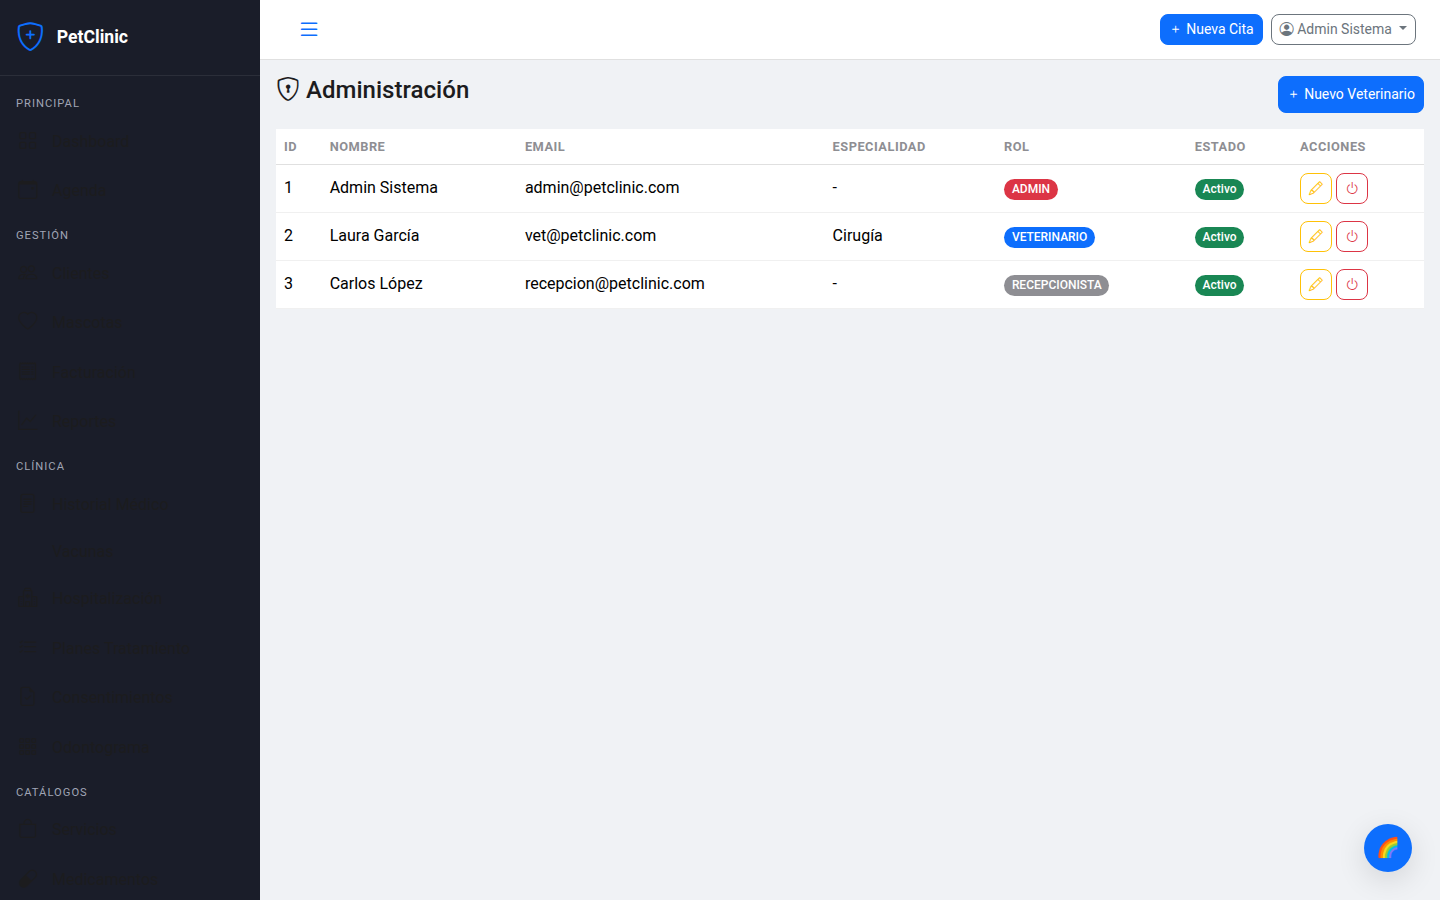
\includegraphics[width=0.9\textwidth]{images/16-admin-veterinarios}
    \caption{Gesti\'on de veterinarios desde el panel de administraci\'on}
    \label{fig:admin}
\end{figure}

\section{M\'odulo de Clientes}

Registro y gesti\'on de due\~nos de mascotas:

\begin{itemize}
    \item Registro con datos de contacto y direcci\'on.
    \item B\'usqueda por nombre, apellido o email.
    \item Portal web para clientes (citas, facturas, historial).
    \item Vista detallada con mascotas asociadas.
\end{itemize}

\section{M\'odulo de Mascotas}

Registro detallado de pacientes con informaci\'on cl\'inica completa:

\begin{itemize}
    \item Informaci\'on completa: especie, raza, color, g\'enero, peso.
    \item Control de alergias y condiciones m\'edicas.
    \item Vista unificada con citas, historial, vacunas y planes.
    \item Integraci\'on con odontograma dental.
\end{itemize}

\section{M\'odulo de Citas}

Agendamiento con calendario interactivo y notificaciones en tiempo real:

\begin{itemize}
    \item Calendario FullCalendar con vistas mensual, semanal y diaria.
    \item Validaci\'on autom\'atica de disponibilidad (evita solapamientos usando JPQL).
    \item Estados: Programada $\rightarrow$ Confirmada $\rightarrow$ En Curso $\rightarrow$ Completada.
    \item Cancelaci\'on con motivo obligatorio.
    \item Notificaciones en tiempo real v\'ia WebSocket (STOMP sobre SockJS).
    \item Arrastrar y soltar para reprogramar citas.
    \item Recordatorio por email al crear la cita.
\end{itemize}

\section{M\'odulo de Facturaci\'on}

Facturaci\'on completa con control de inventario y pagos parciales:

\begin{itemize}
    \item Facturas con items mixtos (servicios + medicamentos).
    \item C\'alculo autom\'atico de subtotales, descuentos y total.
    \item Registro de pagos parciales con control de saldo pendiente.
    \item Estados: Pendiente $\rightarrow$ Pagada Parcial $\rightarrow$ Pagada $\rightarrow$ Anulada.
    \item Descuento autom\'atico de stock al incluir medicamentos.
    \item Generaci\'on de PDF con iText 7 (formato profesional con tabla de items).
    \item Integraci\'on con Stripe para pagos en l\'inea.
\end{itemize}

\section{M\'odulo de Servicios}

Cat\'alogo de servicios ofrecidos por la cl\'inica:

\begin{itemize}
    \item CRUD completo con precio base y c\'odigo interno.
    \item Activaci\'on/desactivaci\'on sin eliminar (\textit{soft delete}).
\end{itemize}

\begin{figure}[H]
    \centering
    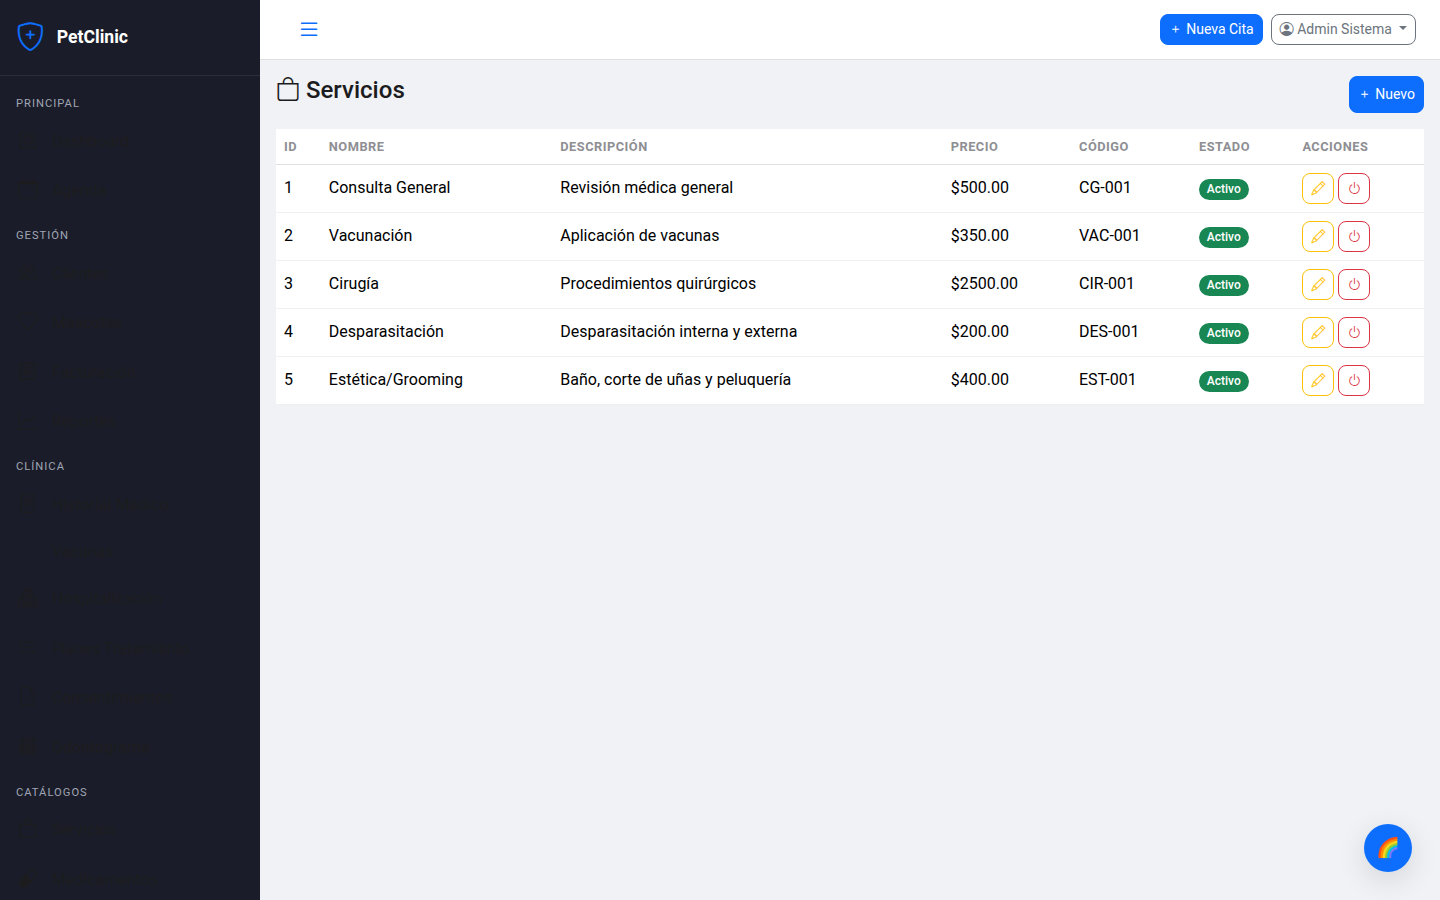
\includegraphics[width=0.9\textwidth]{images/14-servicios}
    \caption{Cat\'alogo de servicios con precios y activaci\'on}
    \label{fig:servicios}
\end{figure}

\section{M\'odulo de Medicamentos e Inventario}

Control de stock con trazabilidad completa de movimientos:

\begin{itemize}
    \item CRUD de medicamentos con unidad de medida y presentaci\'on.
    \item Control de stock m\'inimo con alertas visuales (stock bajo resaltado en rojo).
    \item Trazabilidad: cada movimiento registra tipo (entrada, salida, ajuste), cantidad, fecha y usuario.
    \item Descuento autom\'atico al facturar medicamentos.
    \item Vista de stock bajo (medicamentos con stock menor o igual al m\'inimo configurado).
\end{itemize}

\begin{figure}[H]
    \centering
    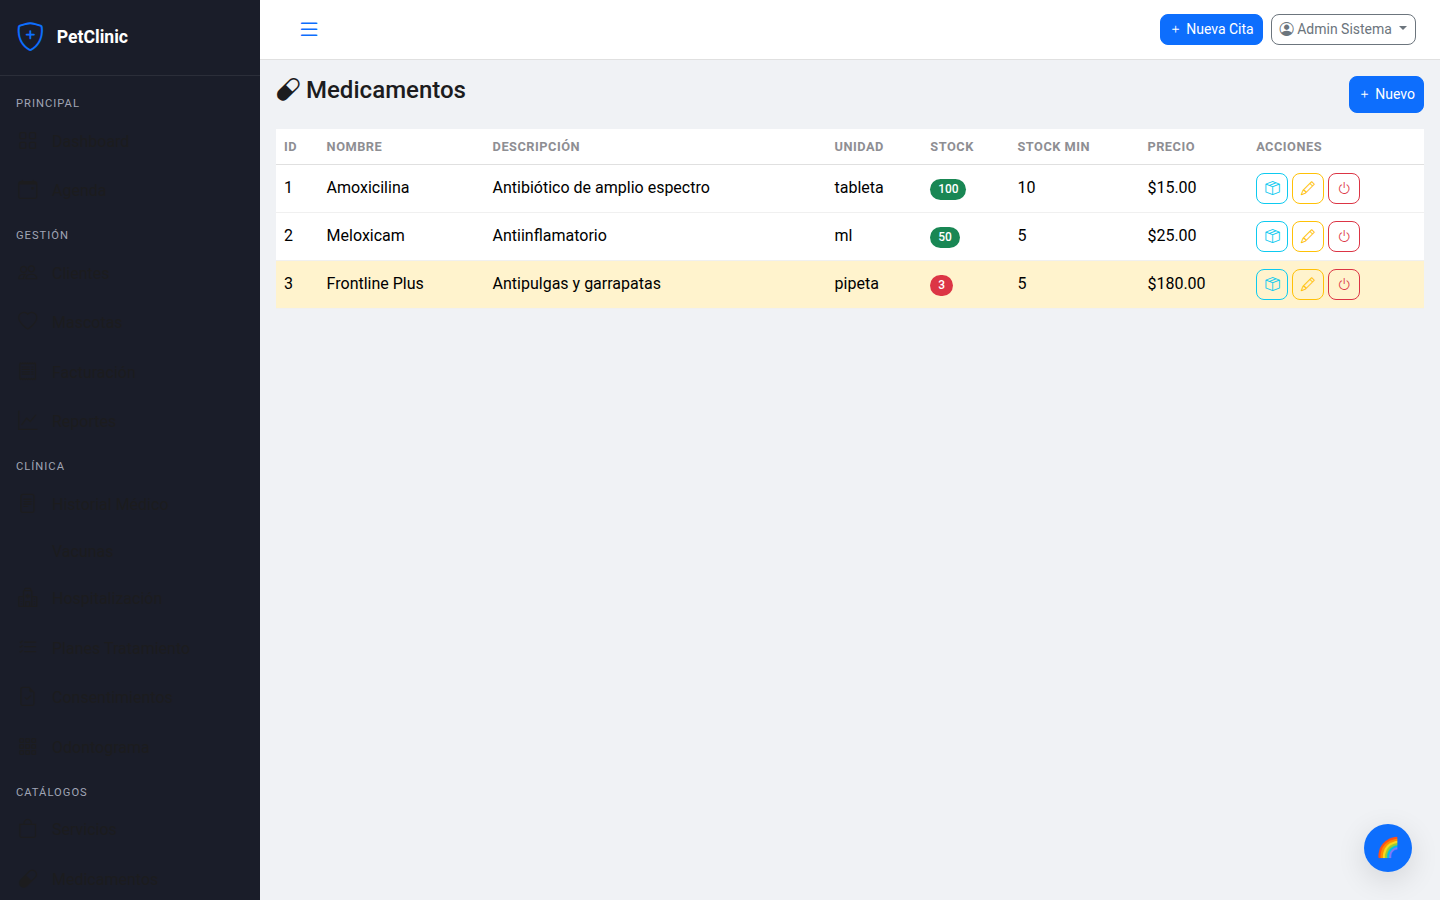
\includegraphics[width=0.9\textwidth]{images/15-medicamentos}
    \caption{Inventario de medicamentos con control de stock}
    \label{fig:medicamentos}
\end{figure}

\section{M\'odulo de Historial M\'edico}

Notas detalladas de consulta por mascota con orden cronol\'ogico:

\begin{itemize}
    \item Registro de motivo, diagn\'ostico, procedimiento y medicaci\'on recetada.
    \item Vinculaci\'on a citas espec\'ificas para contexto completo.
    \item Historial cronol\'ogico completo por mascota con b\'usqueda por fecha.
\end{itemize}

\begin{figure}[H]
    \centering
    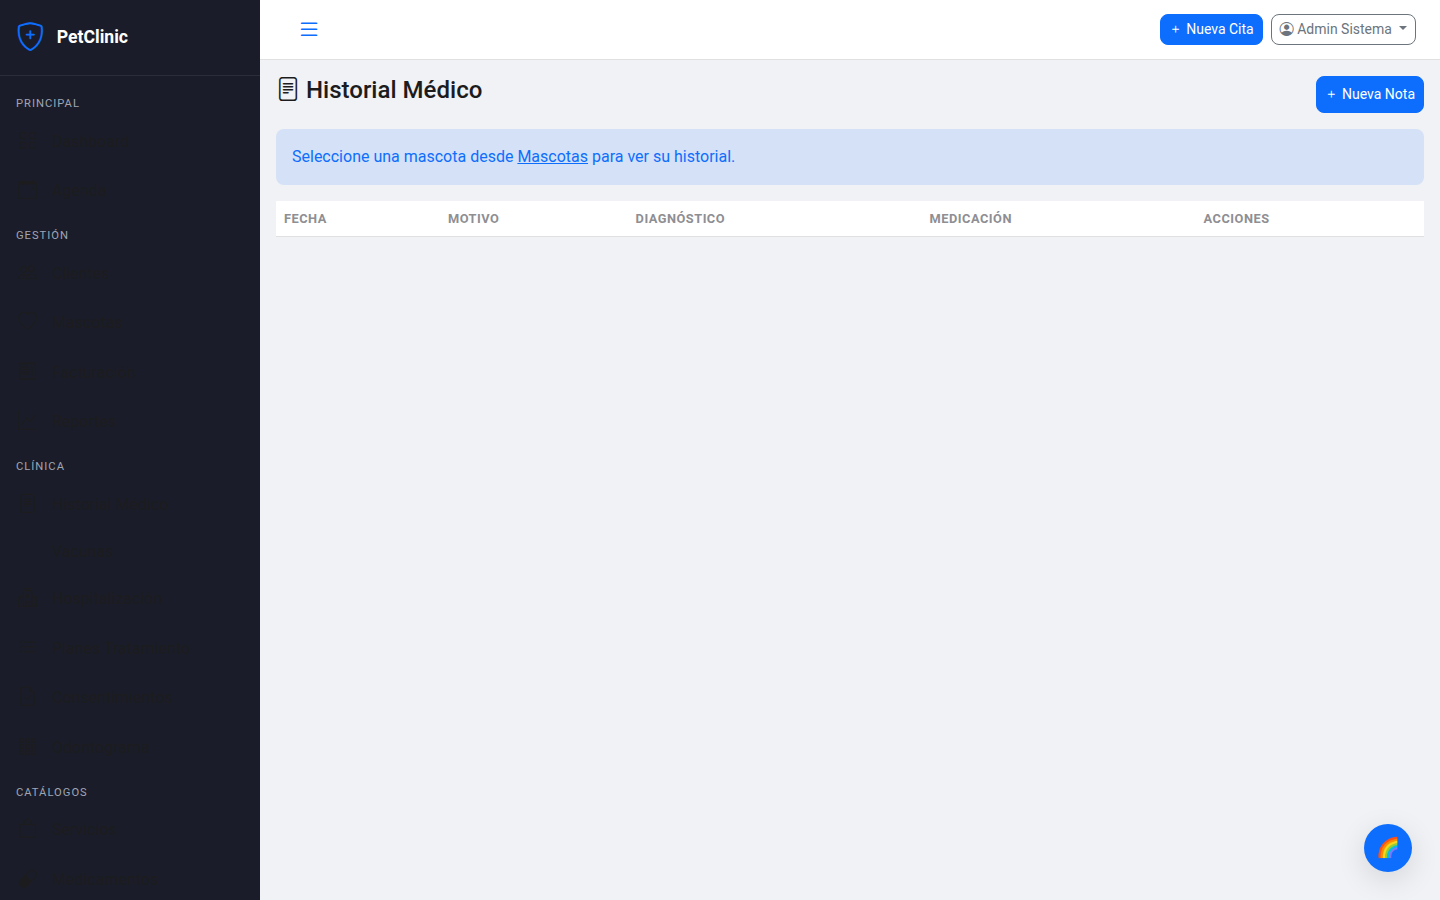
\includegraphics[width=0.9\textwidth]{images/08-historial-medico}
    \caption{Historial m\'edico de mascota con notas de consulta}
    \label{fig:historial}
\end{figure}

\section{M\'odulo de Vacunas}

Control de vacunaci\'on con alertas autom\'aticas por email:

\begin{itemize}
    \item Registro con nombre de vacuna, fecha de aplicaci\'on y pr\'oxima dosis.
    \item Control de lote y fabricante para trazabilidad.
    \item Alertas autom\'aticas por email: vacunas pr\'oximas a vencer (08:00) y vencidas (09:00).
    \item Tareas programadas con \texttt{@Scheduled} y cron expressions.
    \item Integraci\'on con JavaMailSender para env\'io de correos HTML con plantillas.
\end{itemize}

\begin{figure}[H]
    \centering
    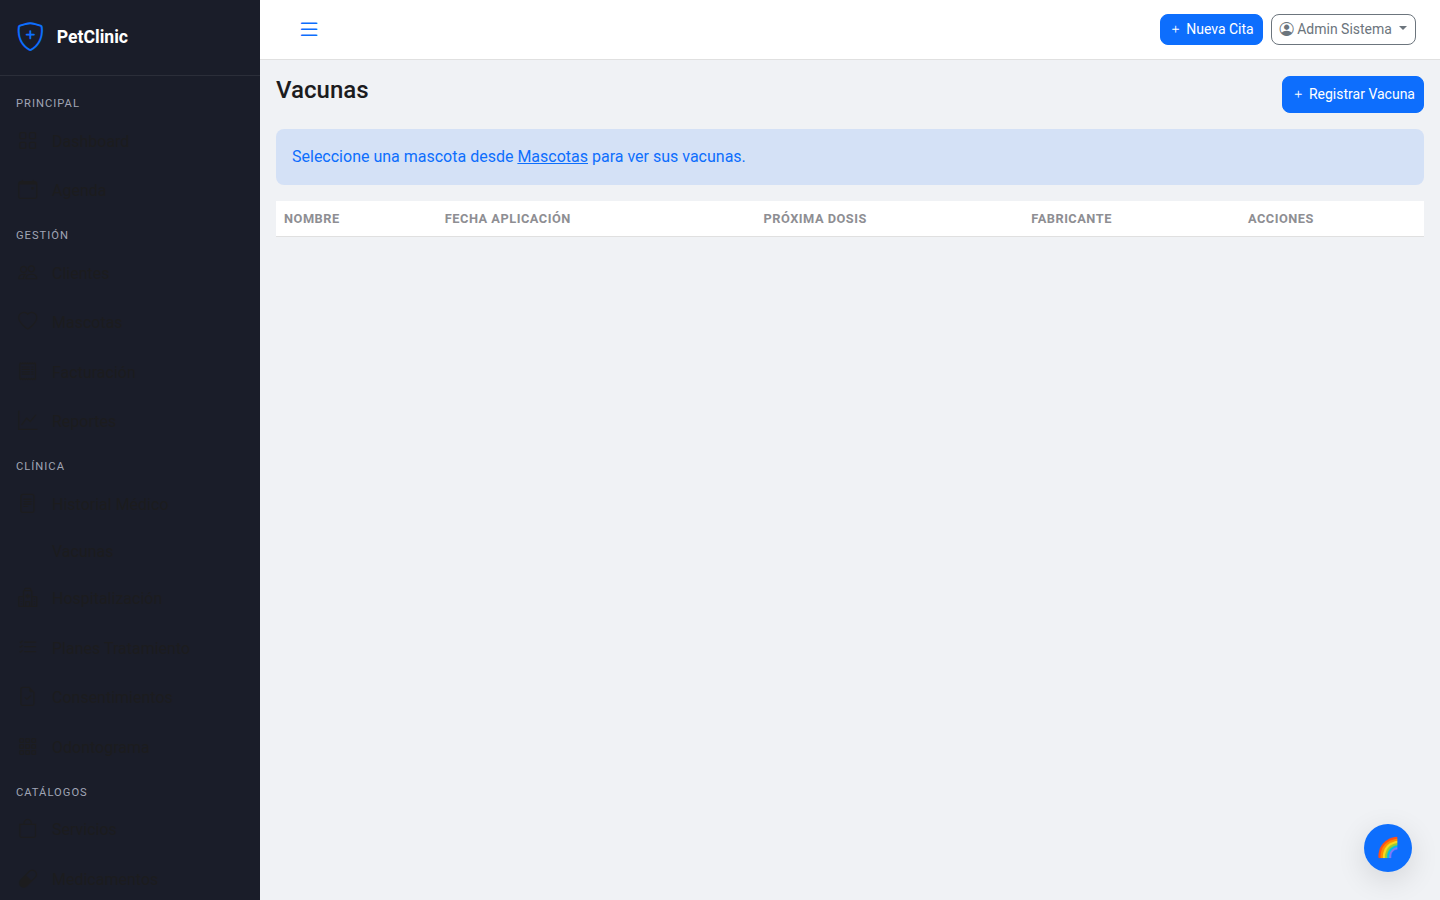
\includegraphics[width=0.9\textwidth]{images/09-vacunas}
    \caption{Registro de vacunas por mascota con alertas}
    \label{fig:vacunas}
\end{figure}

\section{M\'odulo de Hospitalizaci\'on}

Gesti\'on de pacientes hospitalizados con control de ingresos y altas:

\begin{itemize}
    \item Ingreso con asignaci\'on de jaula y motivo de hospitalizaci\'on.
    \item Control de check-in / check-out con fecha y hora exacta.
    \item Estado: Hospitalizado $\rightarrow$ Dado de Alta.
    \item Notas de evoluci\'on durante la estancia.
\end{itemize}

\begin{figure}[H]
    \centering
    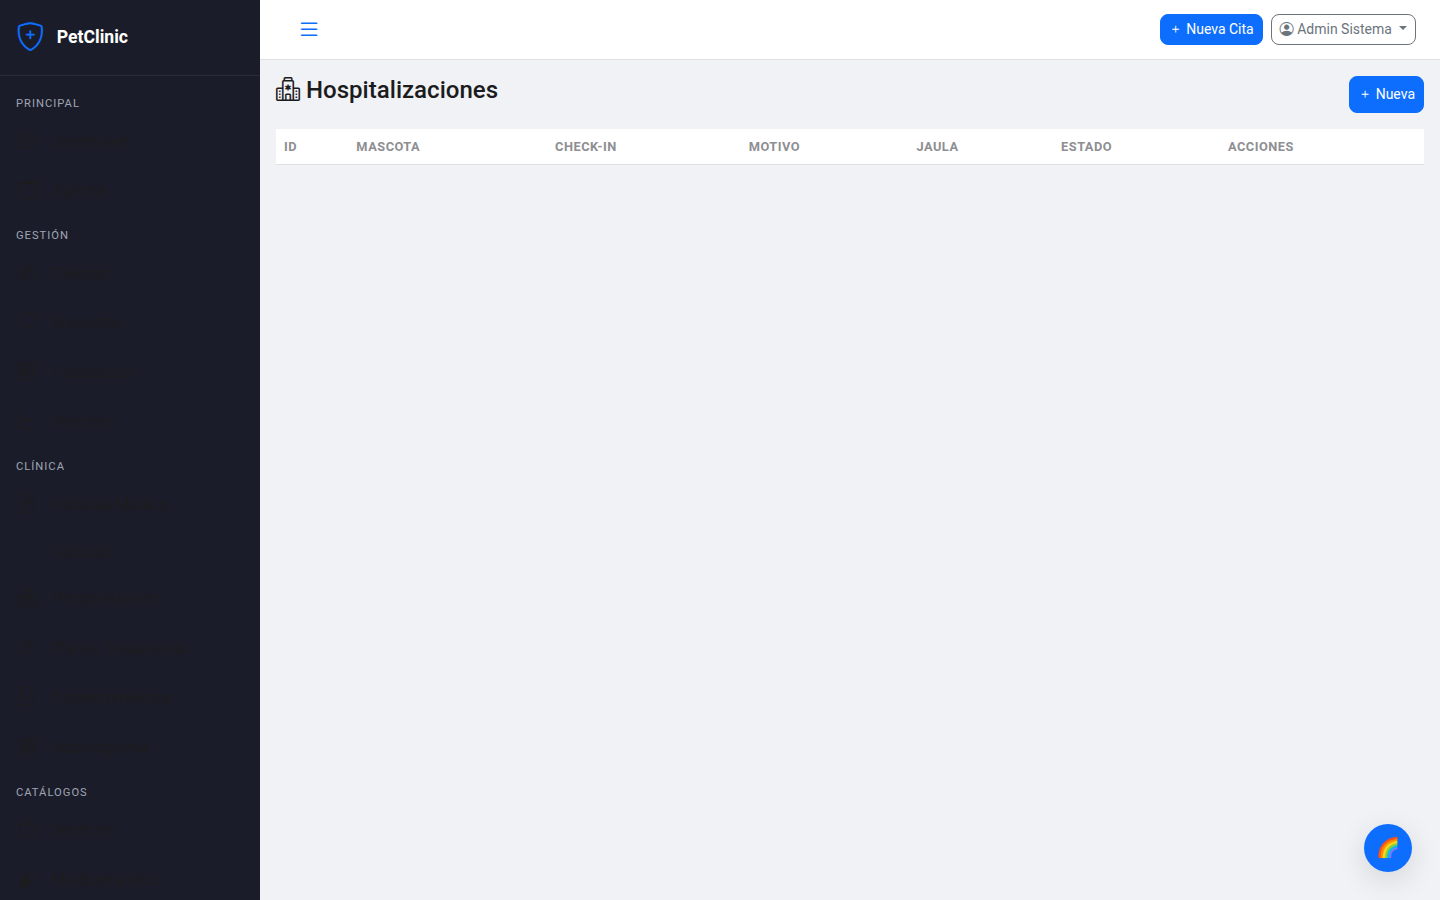
\includegraphics[width=0.9\textwidth]{images/10-hospitalizaciones}
    \caption{Pacientes hospitalizados con control de ingresos}
    \label{fig:hospitalizacion}
\end{figure}

\section{M\'odulo de Planes de Tratamiento}

Planes con pasos secuenciados para seguimiento de tratamientos:

\begin{itemize}
    \item Planes con t\'itulo, descripci\'on y costo estimado total.
    \item Pasos secuenciados con orden, servicio asociado y costo individual.
    \item Seguimiento de avance por paso: Pendiente $\rightarrow$ En Proceso $\rightarrow$ Completado $\rightarrow$ Omitido.
    \item Estados del plan: Activo, Completado, Cancelado.
\end{itemize}

\begin{figure}[H]
    \centering
    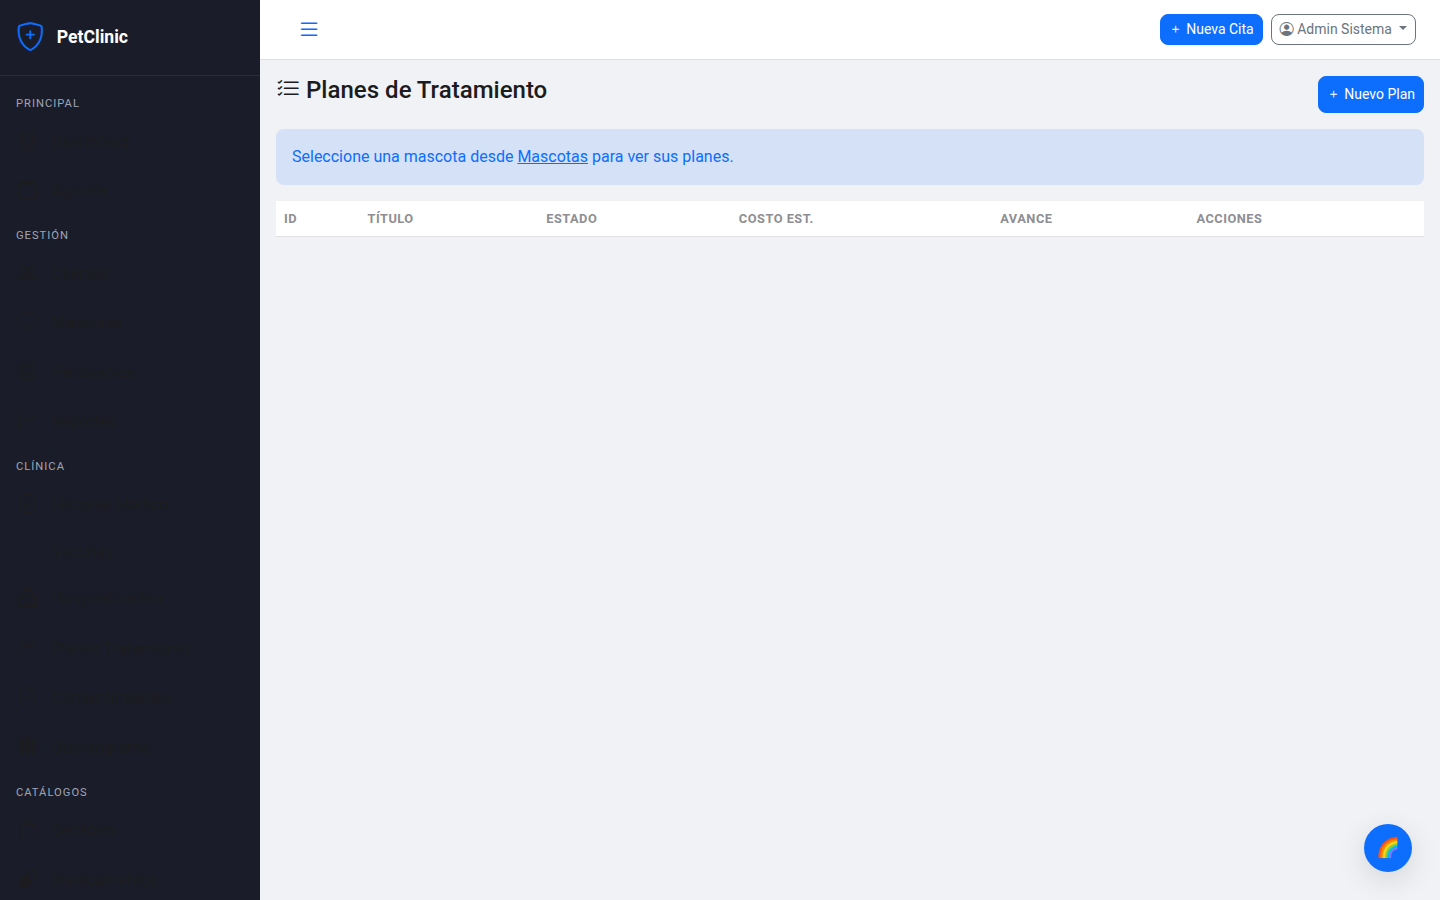
\includegraphics[width=0.9\textwidth]{images/11-planes-tratamiento}
    \caption{Plan de tratamiento con pasos secuenciados y avance}
    \label{fig:planes}
\end{figure}

\section{M\'odulo de Consentimientos Informados}

Documentos legales para procedimientos veterinarios:

\begin{itemize}
    \item Creaci\'on de documentos con t\'itulo, tipo de procedimiento y contenido detallado.
    \item Firma digital con registro de fecha, nombre completo del firmante y relaci\'on con la mascota.
    \item Generaci\'on de PDF profesional para impresi\'on y respaldo.
    \item Control de estado: Pendiente de Firma / Firmado.
\end{itemize}

\begin{figure}[H]
    \centering
    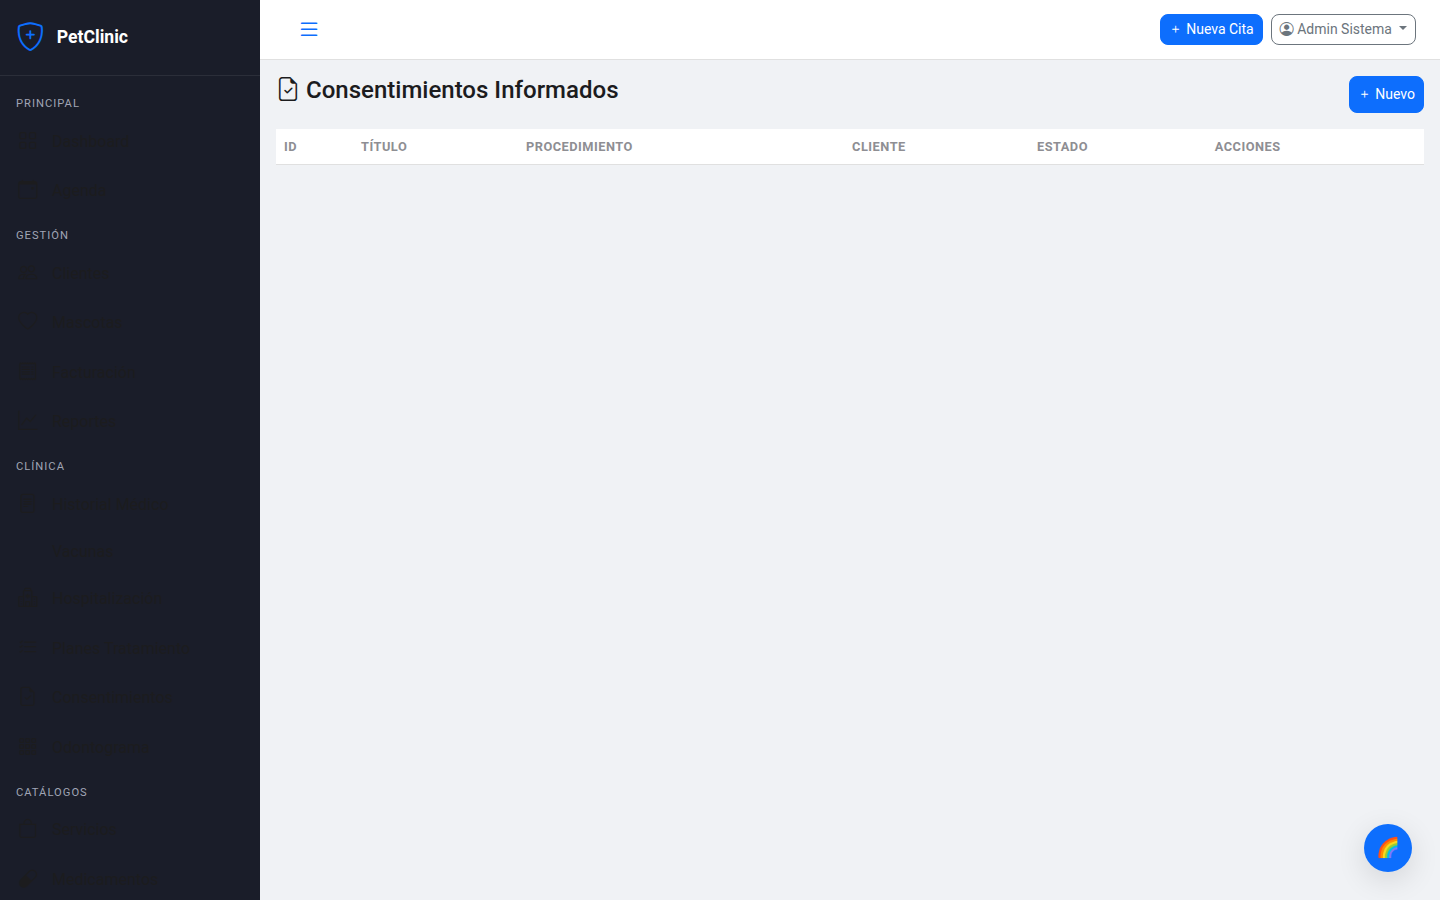
\includegraphics[width=0.9\textwidth]{images/12-consentimientos}
    \caption{Consentimiento informado con firma digital y PDF}
    \label{fig:consentimientos}
\end{figure}

\section{M\'odulo de Odontograma}

Diagrama dental canino interactivo implementado con HTML Canvas:

\begin{itemize}
    \item 42 dientes numerados seg\'un f\'ormula dental canina (I 3/3, C 1/1, P 4/4, M 2/3).
    \item Estados: SANO, T\'ARTARO, CARIES, FRACTURA, AUSENTE, PERIODONTAL, OBTURADO, ENDODONCIA.
    \item Cada estado se representa con un color diferente para identificaci\'on visual r\'apida.
    \item Interfaz interactiva: seleccionar estado en la leyenda y hacer clic en el diente.
    \item Persistencia de m\'ultiples odontogramas por mascota (uno por consulta dental).
\end{itemize}

\section{M\'odulo de Pagos Online (Stripe)}

Integraci\'on con Stripe Payment Intents para pagos en l\'inea:

\begin{itemize}
    \item Creaci\'on de intenci\'on de pago vinculada a una factura espec\'ifica.
    \item Modal simulado cuando Stripe no est\'a configurado (\textit{sandbox mode}).
    \item Webhook \texttt{/api/pagos/stripe/webhook} para confirmaci\'on as\'incrona de pagos.
    \item Actualizaci\'on autom\'atica del estado de la factura al confirmar el pago.
\end{itemize}

\section{M\'odulo de Reserva P\'ublica}

Permite a clientes potenciales agendar citas sin autenticaci\'on:

\begin{itemize}
    \item Listado de veterinarios disponibles con horarios y especialidades.
    \item Visualizaci\'on de slots disponibles por fecha y veterinario.
    \item Validaci\'on de email del cliente contra la base de datos existente.
    \item Creaci\'on de cita como visitante sin necesidad de registro.
\end{itemize}

\section{M\'odulo de Reportes}

An\'alisis de ingresos con visualizaci\'on gr\'afica y exportaci\'on:

\begin{itemize}
    \item Dashboard con 7 indicadores clave del sistema.
    \item Reporte de ingresos por per\'iodo con gr\'afico de barras (Chart.js).
    \item Exportaci\'on a Excel con Apache POI para an\'alisis externo.
    \item Filtro por rango de fechas personalizado.
\end{itemize}

\section{M\'odulo de Auditor\'ia}

Registro de todas las acciones importantes del sistema para cumplimiento y trazabilidad:

\begin{itemize}
    \item Log de acciones CREATE, UPDATE, DELETE con tipo de operaci\'on.
    \item Detalle de entidad afectada y usuario responsable.
    \item Registro de direcci\'on IP del cliente.
    \item Visualizaci\'on en tabla cronol\'ogica con filtros por entidad y fecha.
\end{itemize}

\begin{figure}[H]
    \centering
    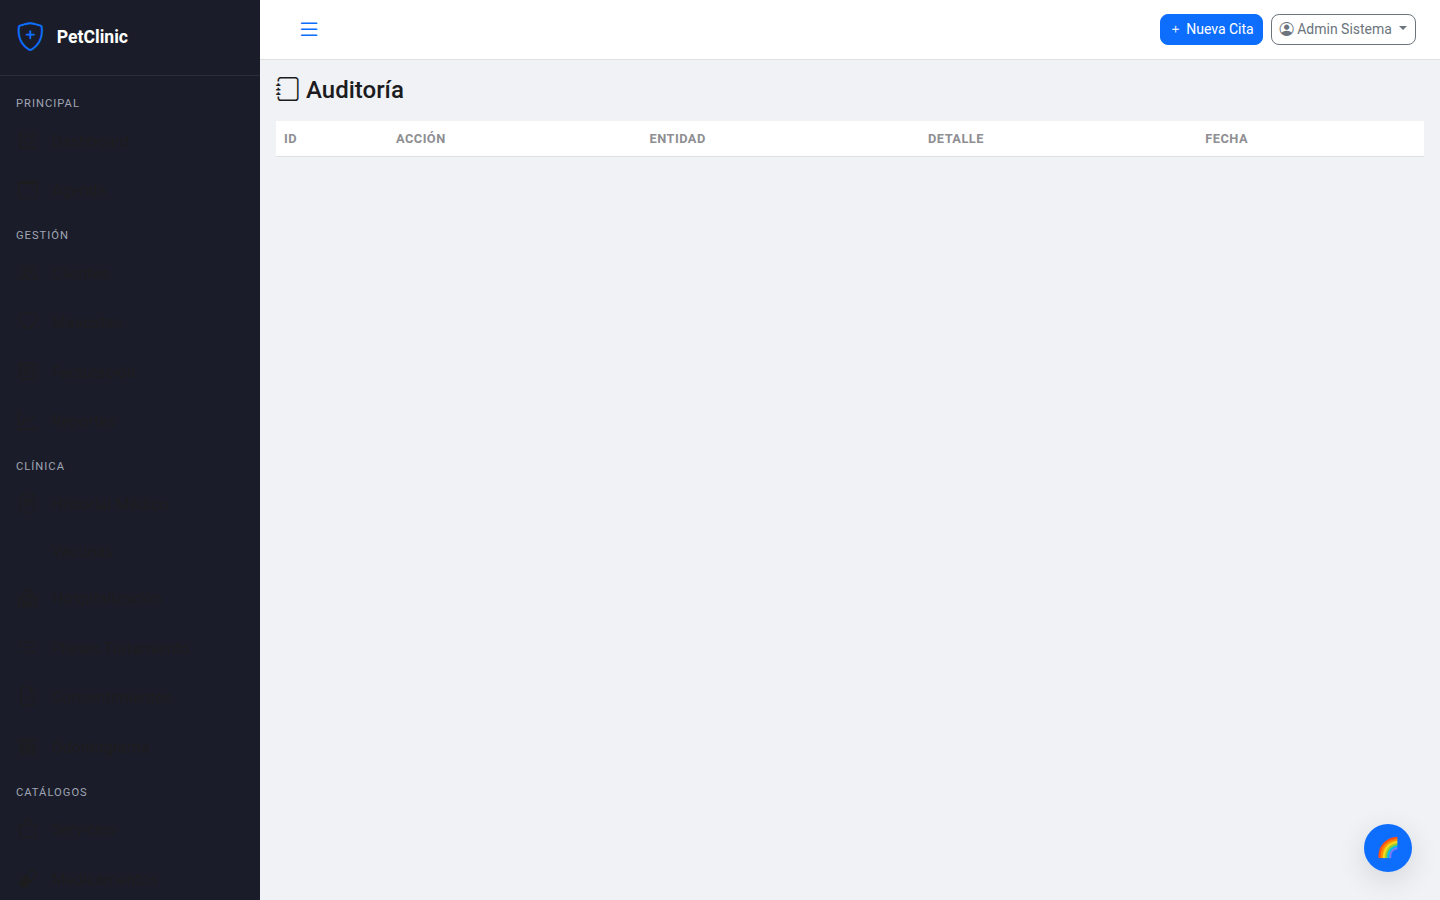
\includegraphics[width=0.9\textwidth]{images/17-auditoria}
    \caption{Log de auditor\'ia con acciones del sistema}
    \label{fig:auditoria2}
\end{figure}

\section{M\'odulo de Configuraci\'on}

Panel de configuraci\'on general del sistema:

\begin{itemize}
    \item Configuraci\'on de datos de la cl\'inica (nombre, direcci\'on, tel\'efono, email).
    \item Configuraci\'on de par\'ametros de facturaci\'on (impuestos, formato de n\'umero).
    \item Configuraci\'on de notificaciones (activar/desactivar alertas por email).
\end{itemize}

\begin{figure}[H]
    \centering
    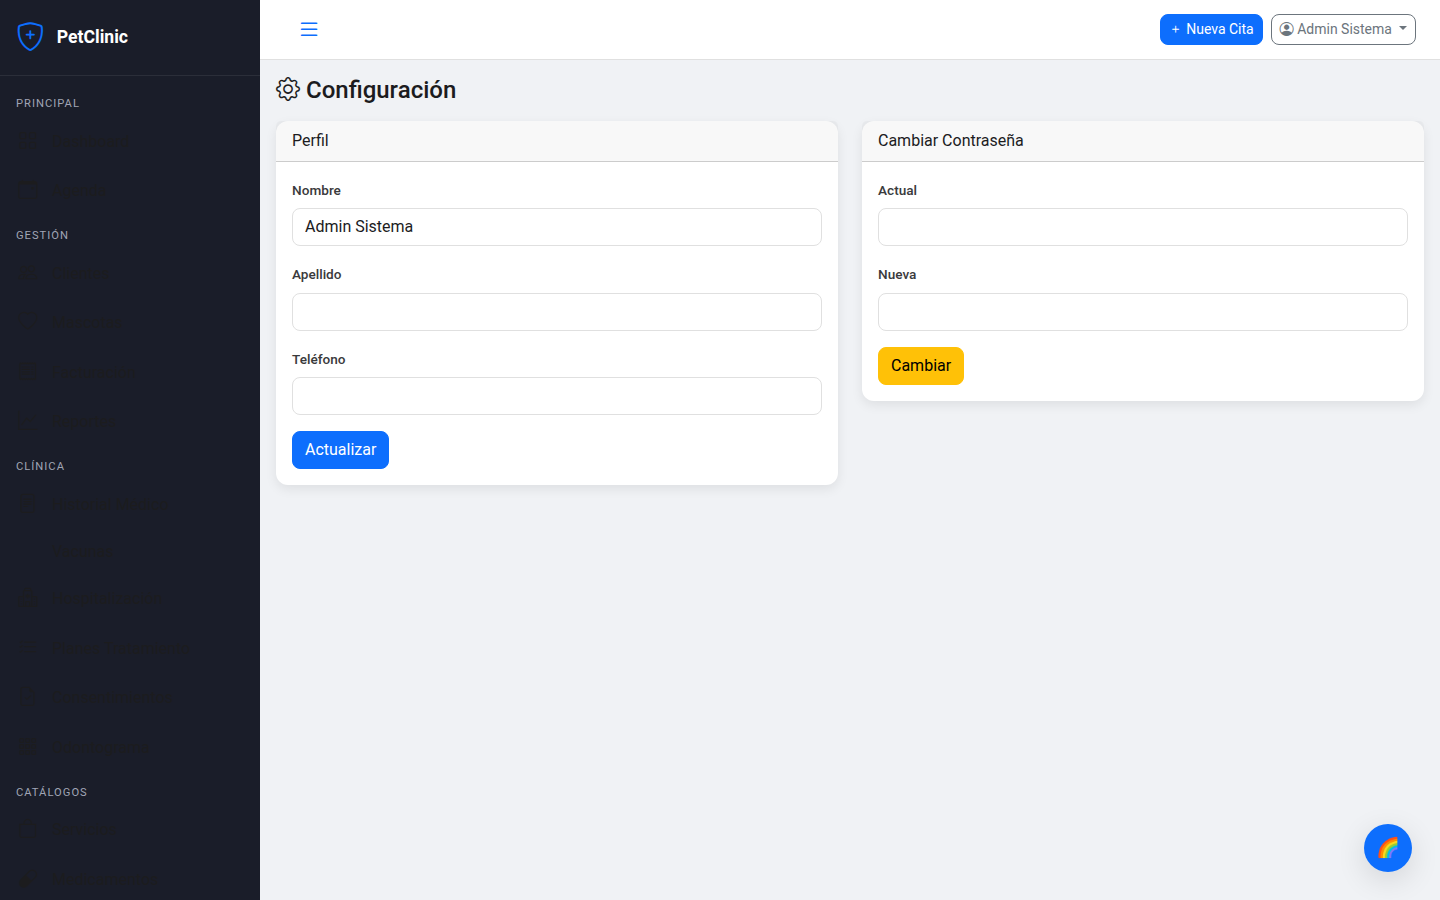
\includegraphics[width=0.9\textwidth]{images/18-configuracion}
    \caption{Panel de configuraci\'on general del sistema}
    \label{fig:config}
\end{figure}

\section{M\'odulo de Notificaciones}

Sistema de alertas multicanal con tareas programadas:

\begin{itemize}
    \item Alertas de vacunaci\'on por email (vacunas pr\'oximas a vencer y vencidas).
    \item Notificaciones autom\'aticas diarias v\'ia \texttt{@Scheduled} a las 08:00 y 09:00.
    \item Recordatorios de citas por email al momento de creaci\'on.
    \item Notificaciones de facturaci\'on (factura creada, pago recibido).
    \item Integraci\'on con JavaMailSender (SMTP) y plantillas HTML personalizables.
\end{itemize}

\begin{lstlisting}[language=Java, caption=Programaci\'on de alertas de vacunaci\'on]
@Component
public class VacunaScheduler {

    @Scheduled(cron = "0 0 8 * * ?")  // 08:00 todos los dias
    public void alertarProximasVacunas() {
        LocalDate hoy = LocalDate.now();
        LocalDate enDosSemanas = hoy.plusDays(14);
        List<Vacuna> proximas = vacunaRepo
            .findByFechaProximaDosisBetween(hoy, enDosSemanas);
        for (Vacuna v : proximas) {
            notificacionService.enviarAlertaVacunacion(v);
        }
    }

    @Scheduled(cron = "0 0 9 * * ?")  // 09:00 todos los dias
    public void alertarVacunasVencidas() {
        List<Vacuna> vencidas = vacunaRepo
            .findByFechaProximaDosisBefore(LocalDate.now());
        for (Vacuna v : vencidas) {
            notificacionService.enviarAlertaVacunacion(v);
        }
    }
}
\end{lstlisting}

\section{Sistema de Temas}

Personalizaci\'on visual con 8 temas de color intercambiables en tiempo real:

\begin{itemize}
    \item Implementado mediante variables CSS (\textit{Custom Properties}) en el elemento \texttt{:root}.
    \item Persistencia en \texttt{localStorage} para recordar el tema entre sesiones.
    \item Aplicaci\'on en tiempo real sin recarga de p\'agina.
    \item Bot\'on flotante en esquina inferior derecha con selector de temas.
    \item Integraci\'on con FullCalendar (actualiza colores del calendario al cambiar tema).
\end{itemize}

\section{Credenciales de Prueba}

\begin{longtable}{|p{3cm}|p{4cm}|p{3cm}|p{4cm}|}
\hline
\textbf{Rol} & \textbf{Email} & \textbf{Password} & \textbf{Descripci\'on} \\
\hline
ADMIN & admin@petclinic.com & Admin123 & Acceso total al sistema \\
VETERINARIO & vet@petclinic.com & Vet123 & Gesti\'on cl\'inica completa \\
RECEPCIONISTA & recepcion@petclinic.com & Recep123 & Lectura y creaci\'on b\'asica \\
CLIENTE & ana@email.com & Ana123 & Portal del cliente \\
\hline
\end{longtable}
